\documentclass[tikz, border=6pt]{standalone}
\usepackage[T1]{fontenc}
\usepackage{lmodern}
\usepackage{amsmath,amssymb,bm}
\usepackage[scaled=0.95]{helvet}
\usetikzlibrary{arrows.meta, positioning}
\definecolor{Blue}{HTML}{3A76D8}
\definecolor{Green}{HTML}{3BA55C}
\definecolor{Orange}{HTML}{EE8133}
\definecolor{Red}{HTML}{DF4B4B}
\definecolor{Ink}{HTML}{1F2937}
\tikzset{
  block/.style={/utils/exec={\colorlet{pytikzarg}{#1}}, draw=pytikzarg!78!black, fill=pytikzarg!14, rounded corners=3pt, align=center, inner sep=5pt, minimum height=8mm, minimum width=20mm},
  block/.default=Blue,
}
\begin{document}
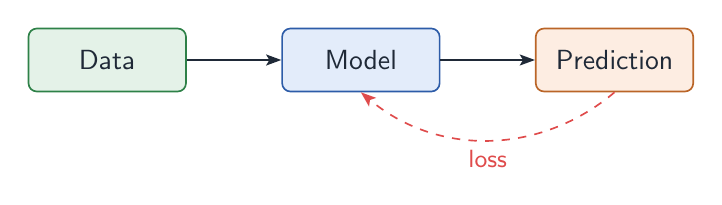
\begin{tikzpicture}[color=Ink, execute at begin picture={\sffamily}, line width=0.6pt, >={Stealth[length=5.5pt, width=4pt, inset=1.2pt]}, line join=round]
  \node[block=Green] (n1) {Data};
  \node[block, right=1.2cm of n1] (n2) {Model};
  \node[block=Orange, right=1.2cm of n2] (n3) {Prediction};
  \draw[->] (n1) -- (n2);
  \draw[->] (n2) -- (n3);
  \draw[->, dashed, color=Red] (n3.south) to[bend left=40] node[pos=0.5, auto, font=\small] {loss}
      (n2.south);
\end{tikzpicture}
\end{document}
